\usetikzlibrary{arrows.meta,calc}
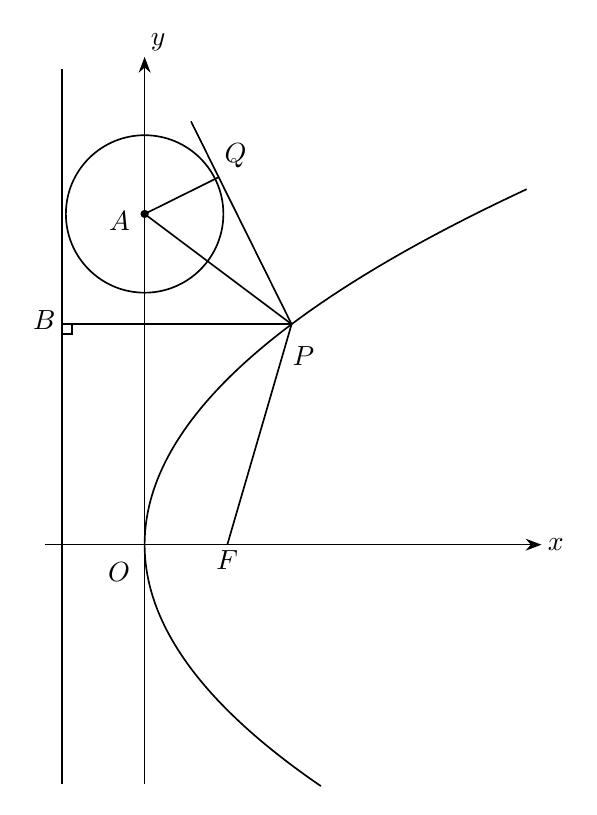
\begin{tikzpicture}[x=1.05cm,y=1.05cm,line width=.6pt,>=Stealth,font=\normalsize]
\coordinate (A) at (0,4);
\coordinate (F) at (1,0);
\coordinate (P) at (1.7778,2.6667);
\coordinate (B) at (-1,2.6667);
\coordinate (Q) at (0.8958,4.4444);
\coordinate (Ttop) at (0.5607,5.12);
\coordinate (Ltop) at (-1,5.75);
\coordinate (Lbot) at (-1,-2.9);
\draw (A) circle[radius=1cm];
\draw[domain=-2.92:4.30,samples=161] plot ({\x*\x/4},{\x});
\draw (Ltop)--(Lbot);
\draw (P)--(B);
\draw (P)--(A);
\draw (Ttop)--(P);
\draw (P)--(F);
\draw (A)--(Q);
\draw (B)--(-0.88,2.6667)--(-0.88,2.5467)--(-1,2.5467);
\fill (A) circle (1.5pt);
\draw[->] (-1.2,0)--(4.8,0) node[right,inner sep=2pt] {$x$};
\draw[->] (0,-2.9)--(0,5.9) node[above right,inner sep=2pt] {$y$};
\node[left,inner sep=2pt] at (-0.1,3.92) {$A$};
\node[inner sep=2pt] at (1.1,4.7) {$Q$};
\node[inner sep=2pt] at (1.92,2.28) {$P$};
\node[left,inner sep=2pt] at (-1,2.72) {$B$};
\node[below left,inner sep=2pt] at (-0.1,-0.14) {$O$};
\node[anchor=north,inner sep=0pt,yshift=-2pt] at (F) {$F$};
\end{tikzpicture}
